% @Author: AnthonyKenny98
% @Date:   2020-04-06 09:45:02
% @Last Modified by:   AnthonyKenny98
% @Last Modified time: 2020-04-06 11:28:04
The method of edge collision detection in this project's implementation of \gls{RRT} relies on detecting segment-plane intersections. The planes are always set up to be parallel with either the $x-y$ plane, the $x-z$ plane, or the $y-z$ plane. Figure \ref{fig:parallelPlanes} demonstrates this point.

\begin{figure}[H]
\begin{centering}
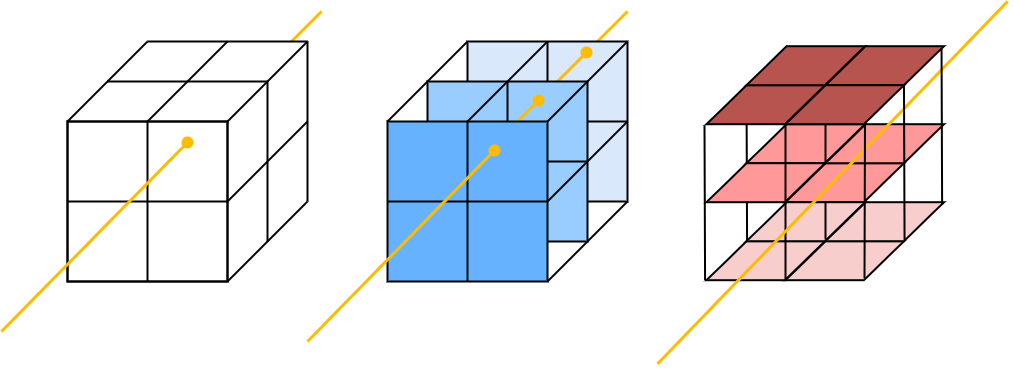
\includegraphics[width=\linewidth]{appendices/rrt/img/planes}
\caption{Using Parallel Planes to determine Edge Collisions with Grids}
\label{fig:parallelPlanes}
\end{centering}
\end{figure}

A plane can be defined by 3 points, $P_a$, $P_b$, and $P_c$. In practice, the points defining a plane parallel to the x-y plane would have the following points:

    $$P_a = (x,y,z)$$
    $$P_b = (x+\Delta x,y,z)$$
    $$P_c = (x,y+\Delta y,z)$$

Two vectors, $\vec{AB}$ and $\vec{AC}$ can be determined.

The normal to the plane is the cross product: 
    $$\vec{AB} \times \vec{AC}$$

And the equation of the plane written as:

    $$a(x-x_0) + b(y-y_0) + c(z-z_0) = 0$$
    $$ax + by + cz = ax_0 + by_0 + cz_0$$

Where $<a,b,c>$ is the normal to the plane and $(x_0, y_0, z_0)$ is one of the points $P_a$, $P_b$, or $P_c$.
The RHS can be set to equal $d$, leaving:

    $$ax + by + cz = d$$

Now, the equation of a line can be written in the form:

    $$ax + by + cz = 0$$

And can be parameterized in the following form:
    $$\begin{cases}
        x = & x_1 + t(x_2 - x_1) \\
        y = & y_1 + t(y_2 - y_1) \\
        z = & z_1 + t(z_2 - z_1) \\

    \end{cases}$$

To find the point of intersection, we substitute the equation of the line into the equation of the plane, yielding:

    $$a(x_1 + t(x_2 - x_1)) + b(x_1 + t(x_2 - x_1)) + c(x_1 + t(x_2 - x_1)) = d$$

Rearranging to find an expression for $t$:

    $$t = \frac{d - (ax_1 + by_1 + cz_1)}{a(x_2-x_1) + b(y_2-y_1) + c(z_2-z_1)}$$

Knowing $t$, we can find the point of intersection, $P_X$ to be:

    $$\begin{cases}
        x_X(t) = & x_1 + t(x_2 - x_1) \\
        y_X(t) = & y_1 + t(y_2 - y_1) \\
        z_X(t) = & z_1 + t(z_2 - z_1) \\
    \end{cases}$$

Finally, the following equalities are evaluated to see if the point lies on the segment:

    $$x_1 \leq x_X \leq x_2$$
    $$y_1 \leq y_X \leq y_2$$
    $$z_1 \leq z_X \leq z_2$$

If so, then the grids corresponding to the point of intersection can be marked as intersected.